\documentclass[letterpaper,12pt]{article}

\usepackage[top=1in, left=1.25in, right=1.25in, bottom=1in]{geometry}
\usepackage[utf8]{inputenc}
\usepackage[T1]{fontenc}
\usepackage[spanish]{babel}
\usepackage{graphicx}
\usepackage{caption}
\usepackage{float}
\usepackage[backend=biber,style=numeric,sorting=none]{biblatex}
\addbibresource{bib/referencias.bib}

\begin{document}

\tableofcontents
\clearpage

\section{Introducción}

\begin{itemize}
\item \textbf{Planteamiento del Problema:} Se busca simular una función \textbf{digestiva} en Java, transformando cadenas de entrada (obtenidas desde args()) en una cadena alfanumérica generada pseudoaleatoriamente. 

\item \textbf{Motivación:} Al realizar esta práctica buscamos lograr una correcta comprensión acerca de lo que realiza una función \textbf{digestiva} y el uso de los \textbf{Hash}. Además de hacer una correcta captura de datos de entrada en el \textbf{Array List}.

\item \textbf{Objetivos:} Comprender la utilidad y las operaciones que realiza una función \textbf{Hash}. Así como hacer un manejo adecuado de cadenas almacenadas en un \textbf{ArrayList} al momento de ejecutar.

\end{itemize}
\section{Marco Teórico}
\textbf{Hash:} Es lo que se obtiene de aplicar una función matemática a una entrada (usualmente una cadena de caracteres), transformando esta en una nueva cadena representativa alfanumérica con una longitud definida.~\cite{hash}

Otra definición: una función computacionalmente eficiente que asigna cadenas de longitud arbitraria a cadenas binarias. Se conocen también como función solo de ida, función unidireccional o función digestiva.~\cite{Funcion_Digestiva}

\textbf{MD5:} Es un protocolo criptográfico que verifica contenido y firmas digitales, basándose en la función Hash para verificar que un archivo es igual que otro, ya que no importa dónde se ejecuten, tendrán la misma clave.~\cite{MD5}


\section{Desarrollo}

\begin{enumerate}

    \item \textbf {Importación de clases:}
    Importamos las clases que utilizaremos en este código, las cuales son:
    \begin{itemize}
        \item \textbf{import java.util.ArrayList; :} 
        Ya que se usa un ArrayList para almacenar las entradas
        \item \textbf{import java.util.HashMap; :} 
        Ya que se utilizará un HashMap para almacenar las parejas clave–valor correspondientes a la cadena de entrada.
        \item \textbf{import java.util.Random; :} 
        Porque se usa Random para generar números pseudoaleatorios a partir de la semilla obtenida de cada palabra ingresada.
    \end{itemize}


    \item \textbf{Creación del Hash:}

   El método \textbf{generaHash} que nos proporcionó el profesor, obtiene una semilla a partir de la suma de los valores numéricos que tiene cada carácter de la cadena de entrada. 
   
   Luego se crea un objeto de tipo \textbf{Random}, y usamos el constructor que recibe una semilla, para que siempre genere el mismo tipo de números con la misma semilla. 

   Después creamos un objeto \textbf{StringBuilder}, este nos permite manejar cadenas de forma mas eficiente.

   Dentro de un ciclo \textbf{for} que itera 32 veces (simulando un \textbf{MD5}), se generan valores aleatorios del 0 al 16 con el objeto \textbf{Random} ya predefinido con una semilla, esto con el objetivo de solo generar valores \textbf{hexadecimales}, y se agregan al objeto \textbf{StringBuilder}, pero antes convirtiendo ese valor a su representación \textbf{hexadecimal}.

   Finalmente se regresa ese valor generado pero en cadena con el método \textbf{toString();}.

   \item \textbf{Desarrollo del main:}

   Dentro del método \textbf{main}, creamos un \textbf{ArrayList} y un \textbf{HashMap} 

   Antes de iniciar cualquier operación en el programa, evaluamos si se ingresó alguna cadena en la ejecución, de no ser así, se imprime un mensaje pidiendo ingresar alguna cadenas al ejecutar y termina la ejecución 
   
   Si el programa continua su ejecución, almacenamos en el \textbf{ArrayList} las cadenas de \textbf{args} ingresadas en la ejecución, y posteriormente iteramos en el \textbf{ArrayList}, convirtiendo cada cadena en una llave con el metodo ya creado \textbf{generaHash}, y después agregando esa llave junto con su cadena al \textbf{hash}.

    \end{enumerate}

\section{Resultados}

\begin{figure}[H]
    \centering
    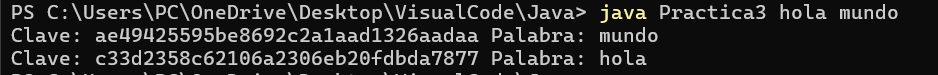
\includegraphics[width=1\textwidth]{Imagenes/ejecucion.png}
    \caption*{Manera correcta de ejecución y salida}
    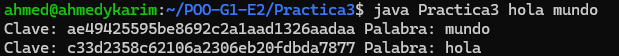
\includegraphics[width=1\textwidth]{Imagenes/hola.png}
    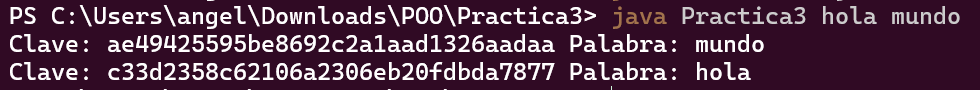
\includegraphics[width=1\textwidth]{Imagenes/image.png}    
    \caption*{Ejecución en otros equipos}
\end{figure}

\clearpage

\section{Conclusiones}
La práctica permitió comprender adecuadamente cómo una función Hash transforma cadenas de texto en claves únicas, las cuales se mantendrán iguales sin importar el equipo donde se realice la ejecución, lo que facilita su uso para identificadores únicos. 

También entendimos el uso y la diferencia entre un \textbf{Hash} y un \textbf{HashMap}, donde en el HashMap se guardan claves únicas con un único valor. Así como también entendimos el uso y las operaciones de un \textbf{ArrayList}.

\printbibliography

\clearpage

\section{Reto para token}

Para asegurarnos que el usuario siempre ingrese 3 valores para calcular la formula general desde la ejecución del programa, pusimos un \textbf{if} que evaluara si el tamaño del arreglo \textbf{args} era diferente de 3, lo que significaba que había ingresado mas o menos valores a los solicitados (a, b , c).

\begin{figure}[H]
    \centering
    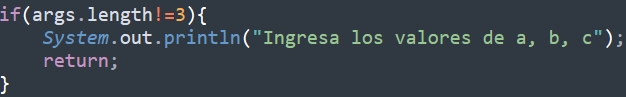
\includegraphics[width=0.5\linewidth]{Imagenes/return.png}
    \caption*{Condicion inicial}
\end{figure}

Luego convertimos los valores que recibe args a double con \textbf{Double.ParseDouble}, para poder utilizarlos en la operaciones, ya que llegan como cadenas

\begin{figure}[H]
    \centering
    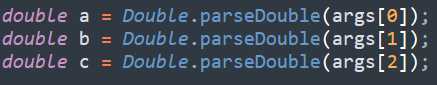
\includegraphics[width=0.5\linewidth]{Imagenes/double.png}
    \caption*{Conversión a double}
\end{figure}

Utilizamos una variable que calculara el determinante para saber si los resultados serian reales o imaginarios, en el caso de los reales, se calcula la formula general directamente y se imprimen los 2 valores de \textbf{x}, considerando los signos. En el caso de ser números complejos, calculamos la parte imaginaria y la parte real en variables diferentes, y luego las imprimimos considerando los signos. 

\begin{figure}[H]
    \centering
    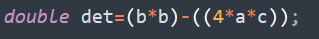
\includegraphics[width=0.5\linewidth]{Imagenes/det.png}
    \caption*{Calculo del determinante}
\end{figure}

Utilizamos los métodos \textbf{Math.abs();} para calcular los números imaginarios cuando era el caso y \textbf{Math.sqrt();} para la raíz de la formula general

\end{document}